% Data Schema — AAPR Platform
% Generated from server/prisma/schema.prisma (source of truth)
\documentclass[tikz,border=10pt]{standalone}
\usepackage[utf8]{inputenc}
\usepackage[T1]{fontenc}
\usepackage{lmodern}
\usetikzlibrary{positioning,arrows.meta,fit,backgrounds,shapes.multipart}

\begin{document}
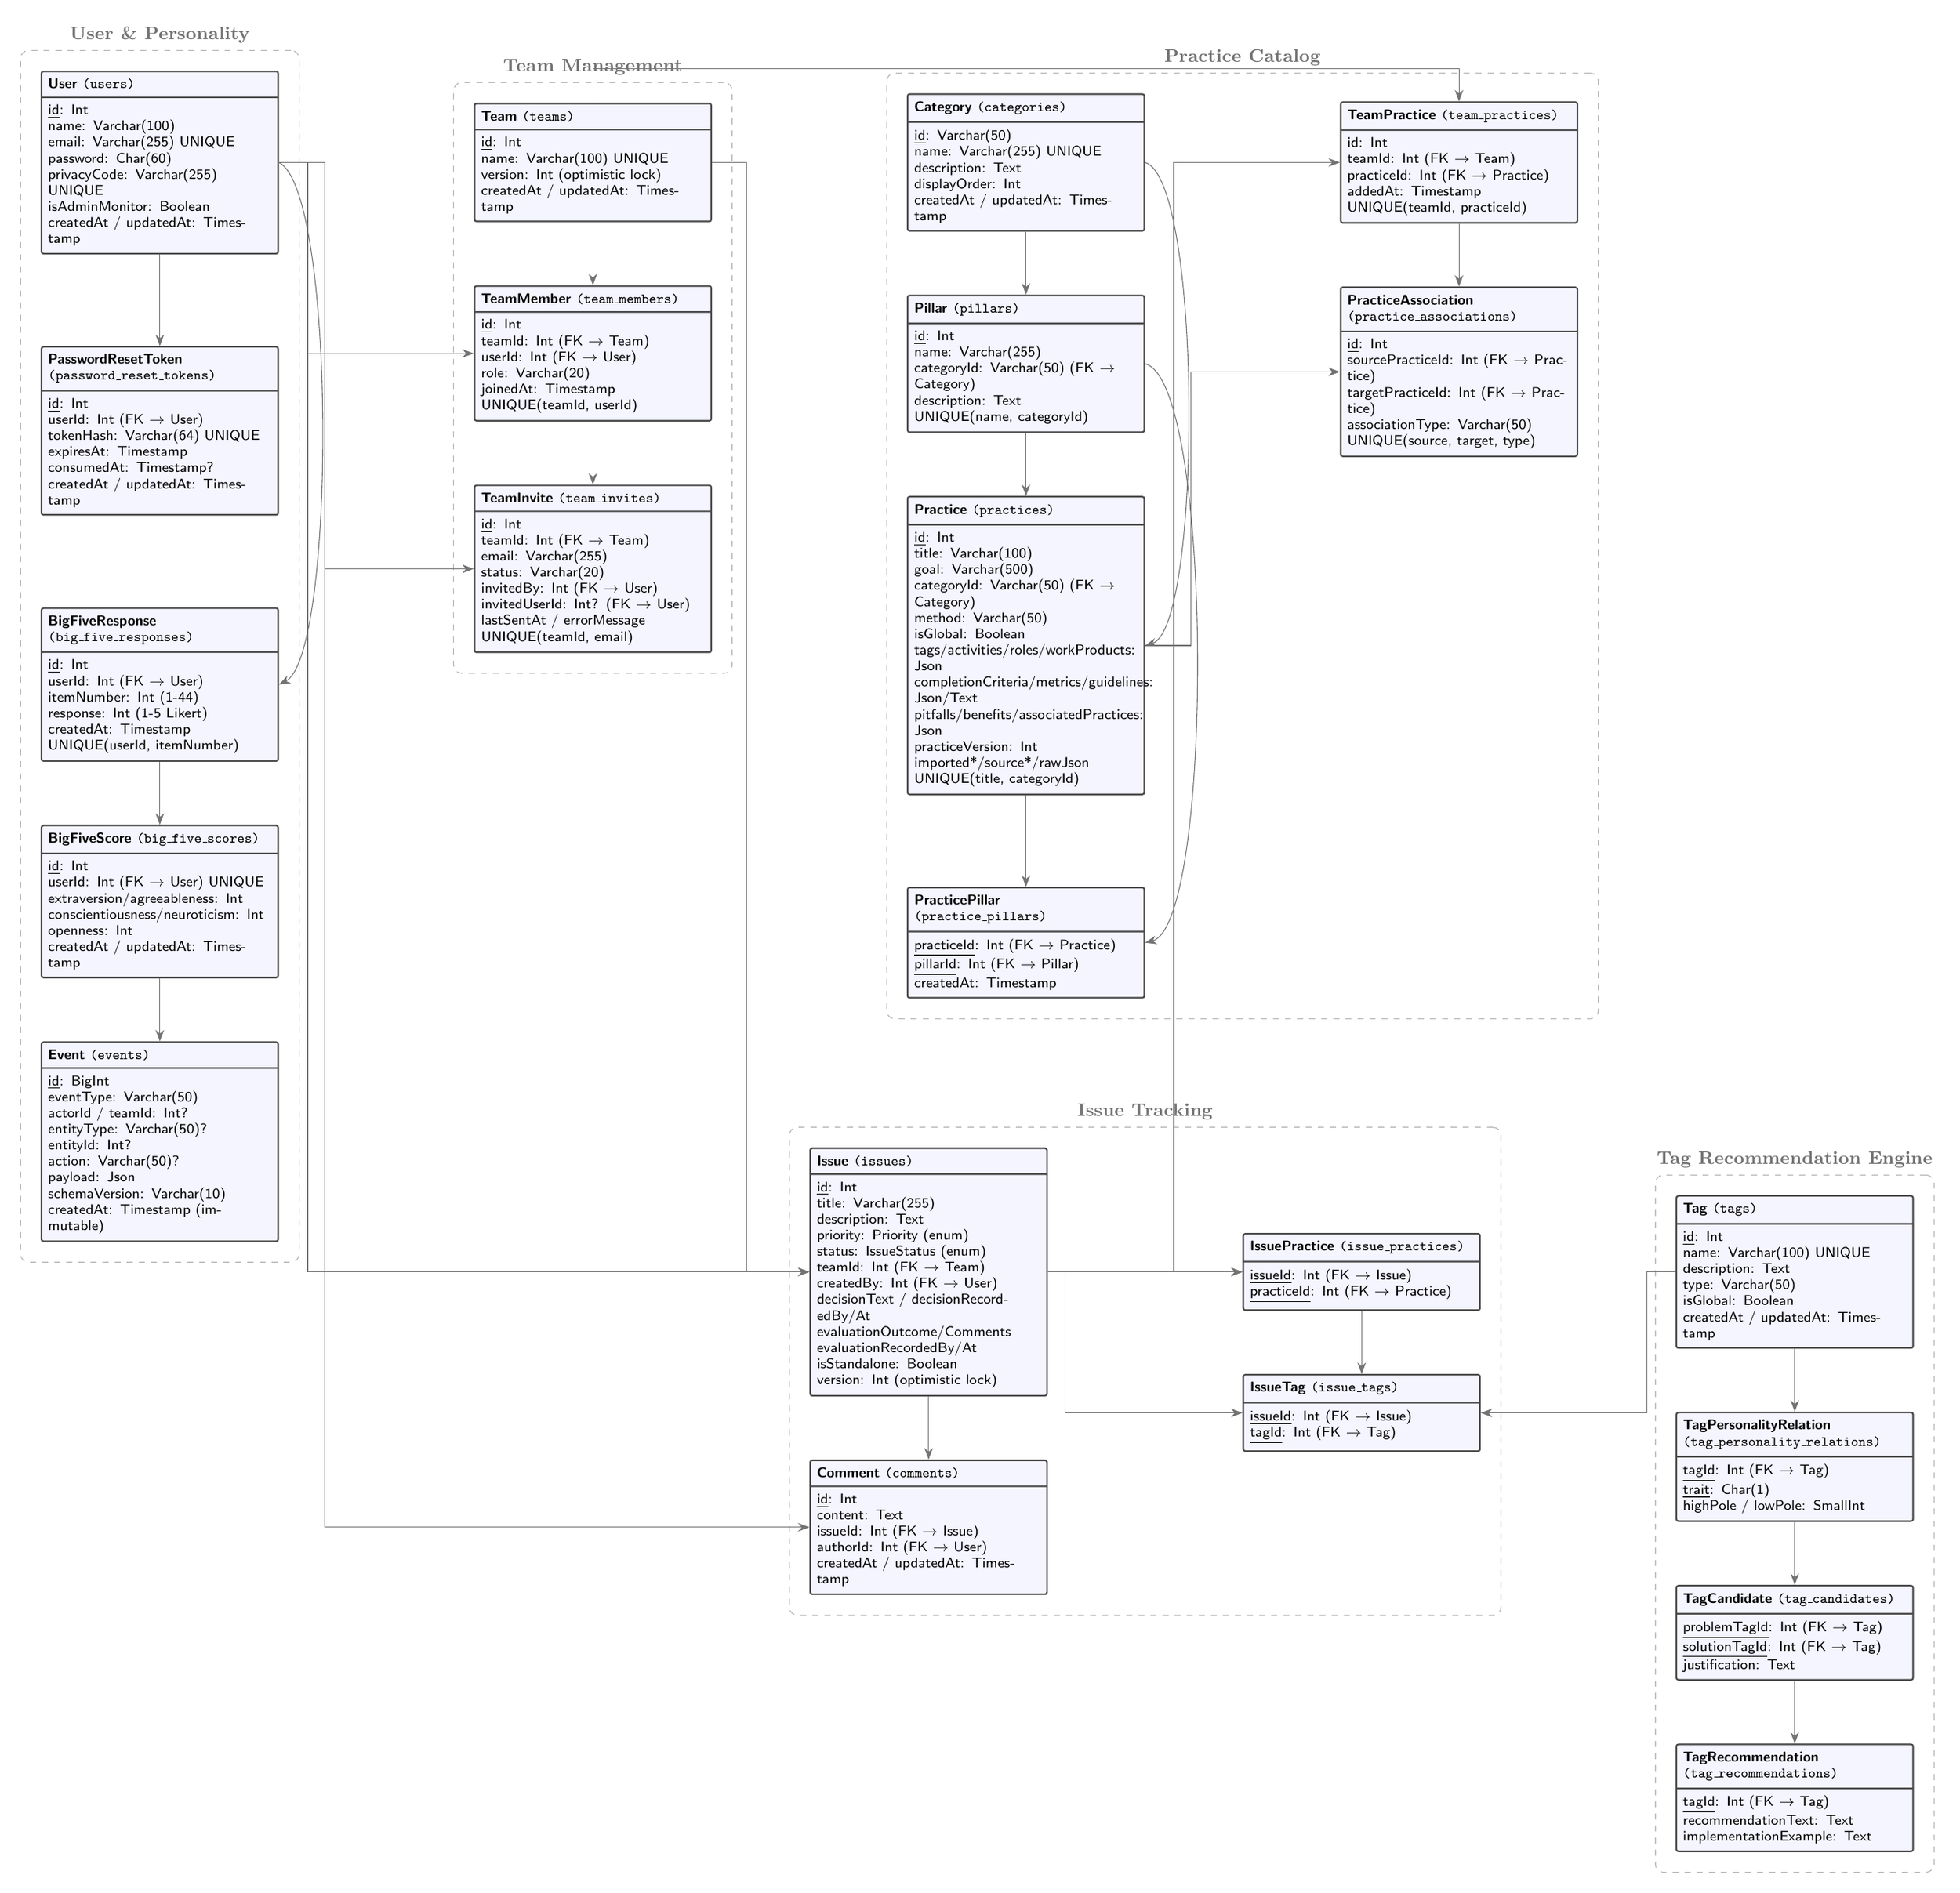
\begin{tikzpicture}[
  font=\sffamily\scriptsize,
  entity/.style={
    rectangle split, rectangle split parts=2,
    rectangle split part align={left,left},
    draw=black!70, thick, rounded corners=1pt,
    fill=blue!4, text width=3.9cm,
    rectangle split part fill={blue!18,white}
  },
  title/.style={font=\bfseries\scriptsize},
  pk/.style={},
  rel/.style={-{Stealth[length=2mm]}, draw=black!55},
  group/.style={draw=black!30, dashed, rounded corners=4pt, inner sep=10pt},
  glabel/.style={font=\bfseries\small, black!55}
]

% =====================================================================
% GROUP 1: USER MANAGEMENT
% =====================================================================
\node[entity] (User) {
  \nodepart{one}\textbf{User} \texttt{(users)}
  \nodepart{two}
  \underline{id}: Int\\
  name: Varchar(100)\\
  email: Varchar(255) UNIQUE\\
  password: Char(60)\\
  privacyCode: Varchar(255) UNIQUE\\
  isAdminMonitor: Boolean\\
  createdAt / updatedAt: Timestamp
};

\node[entity, below=1.6cm of User] (PasswordResetToken) {
  \nodepart{one}\textbf{PasswordResetToken} \texttt{(password\_reset\_tokens)}
  \nodepart{two}
  \underline{id}: Int\\
  userId: Int (FK $\to$ User)\\
  tokenHash: Varchar(64) UNIQUE\\
  expiresAt: Timestamp\\
  consumedAt: Timestamp?\\
  createdAt / updatedAt: Timestamp
};

% =====================================================================
% GROUP 2: TEAM MANAGEMENT
% =====================================================================
\node[entity, right=3.4cm of User] (Team) {
  \nodepart{one}\textbf{Team} \texttt{(teams)}
  \nodepart{two}
  \underline{id}: Int\\
  name: Varchar(100) UNIQUE\\
  version: Int (optimistic lock)\\
  createdAt / updatedAt: Timestamp
};

\node[entity, below=1.1cm of Team] (TeamMember) {
  \nodepart{one}\textbf{TeamMember} \texttt{(team\_members)}
  \nodepart{two}
  \underline{id}: Int\\
  teamId: Int (FK $\to$ Team)\\
  userId: Int (FK $\to$ User)\\
  role: Varchar(20)\\
  joinedAt: Timestamp\\
  UNIQUE(teamId, userId)
};

\node[entity, below=1.1cm of TeamMember] (TeamInvite) {
  \nodepart{one}\textbf{TeamInvite} \texttt{(team\_invites)}
  \nodepart{two}
  \underline{id}: Int\\
  teamId: Int (FK $\to$ Team)\\
  email: Varchar(255)\\
  status: Varchar(20)\\
  invitedBy: Int (FK $\to$ User)\\
  invitedUserId: Int? (FK $\to$ User)\\
  lastSentAt / errorMessage\\
  UNIQUE(teamId, email)
};

% =====================================================================
% GROUP 3: PRACTICE CATALOG
% =====================================================================
\node[entity, right=3.4cm of Team] (Category) {
  \nodepart{one}\textbf{Category} \texttt{(categories)}
  \nodepart{two}
  \underline{id}: Varchar(50)\\
  name: Varchar(255) UNIQUE\\
  description: Text\\
  displayOrder: Int\\
  createdAt / updatedAt: Timestamp
};

\node[entity, below=1.1cm of Category] (Pillar) {
  \nodepart{one}\textbf{Pillar} \texttt{(pillars)}
  \nodepart{two}
  \underline{id}: Int\\
  name: Varchar(255)\\
  categoryId: Varchar(50) (FK $\to$ Category)\\
  description: Text\\
  UNIQUE(name, categoryId)
};

\node[entity, below=1.1cm of Pillar] (Practice) {
  \nodepart{one}\textbf{Practice} \texttt{(practices)}
  \nodepart{two}
  \underline{id}: Int\\
  title: Varchar(100)\\
  goal: Varchar(500)\\
  categoryId: Varchar(50) (FK $\to$ Category)\\
  method: Varchar(50)\\
  isGlobal: Boolean\\
  tags/activities/roles/workProducts: Json\\
  completionCriteria/metrics/guidelines: Json/Text\\
  pitfalls/benefits/associatedPractices: Json\\
  practiceVersion: Int\\
  imported*/source*/rawJson\\
  UNIQUE(title, categoryId)
};

\node[entity, below=1.6cm of Practice] (PracticePillar) {
  \nodepart{one}\textbf{PracticePillar} \texttt{(practice\_pillars)}
  \nodepart{two}
  \underline{practiceId}: Int (FK $\to$ Practice)\\
  \underline{pillarId}: Int (FK $\to$ Pillar)\\
  createdAt: Timestamp
};

\node[entity, right=3.4cm of Category] (TeamPractice) {
  \nodepart{one}\textbf{TeamPractice} \texttt{(team\_practices)}
  \nodepart{two}
  \underline{id}: Int\\
  teamId: Int (FK $\to$ Team)\\
  practiceId: Int (FK $\to$ Practice)\\
  addedAt: Timestamp\\
  UNIQUE(teamId, practiceId)
};

\node[entity, below=1.1cm of TeamPractice] (PracticeAssociation) {
  \nodepart{one}\textbf{PracticeAssociation} \texttt{(practice\_associations)}
  \nodepart{two}
  \underline{id}: Int\\
  sourcePracticeId: Int (FK $\to$ Practice)\\
  targetPracticeId: Int (FK $\to$ Practice)\\
  associationType: Varchar(50)\\
  UNIQUE(source, target, type)
};

% =====================================================================
% GROUP 4: ISSUE TRACKING
% =====================================================================
\node[entity, below=2.6cm of PracticePillar, xshift=-1.7cm] (Issue) {
  \nodepart{one}\textbf{Issue} \texttt{(issues)}
  \nodepart{two}
  \underline{id}: Int\\
  title: Varchar(255)\\
  description: Text\\
  priority: Priority (enum)\\
  status: IssueStatus (enum)\\
  teamId: Int (FK $\to$ Team)\\
  createdBy: Int (FK $\to$ User)\\
  decisionText / decisionRecordedBy/At\\
  evaluationOutcome/Comments\\
  evaluationRecordedBy/At\\
  isStandalone: Boolean\\
  version: Int (optimistic lock)
};

\node[entity, below=1.1cm of Issue] (Comment) {
  \nodepart{one}\textbf{Comment} \texttt{(comments)}
  \nodepart{two}
  \underline{id}: Int\\
  content: Text\\
  issueId: Int (FK $\to$ Issue)\\
  authorId: Int (FK $\to$ User)\\
  createdAt / updatedAt: Timestamp
};

\node[entity, right=3.4cm of Issue] (IssuePractice) {
  \nodepart{one}\textbf{IssuePractice} \texttt{(issue\_practices)}
  \nodepart{two}
  \underline{issueId}: Int (FK $\to$ Issue)\\
  \underline{practiceId}: Int (FK $\to$ Practice)
};

\node[entity, below=1.1cm of IssuePractice] (IssueTag) {
  \nodepart{one}\textbf{IssueTag} \texttt{(issue\_tags)}
  \nodepart{two}
  \underline{issueId}: Int (FK $\to$ Issue)\\
  \underline{tagId}: Int (FK $\to$ Tag)
};

% =====================================================================
% GROUP 5: TAG / RECOMMENDATION ENGINE
% =====================================================================
\node[entity, right=3.4cm of IssuePractice] (Tag) {
  \nodepart{one}\textbf{Tag} \texttt{(tags)}
  \nodepart{two}
  \underline{id}: Int\\
  name: Varchar(100) UNIQUE\\
  description: Text\\
  type: Varchar(50)\\
  isGlobal: Boolean\\
  createdAt / updatedAt: Timestamp
};

\node[entity, below=1.1cm of Tag] (TagPersonalityRelation) {
  \nodepart{one}\textbf{TagPersonalityRelation} \texttt{(tag\_personality\_relations)}
  \nodepart{two}
  \underline{tagId}: Int (FK $\to$ Tag)\\
  \underline{trait}: Char(1)\\
  highPole / lowPole: SmallInt
};

\node[entity, below=1.1cm of TagPersonalityRelation] (TagCandidate) {
  \nodepart{one}\textbf{TagCandidate} \texttt{(tag\_candidates)}
  \nodepart{two}
  \underline{problemTagId}: Int (FK $\to$ Tag)\\
  \underline{solutionTagId}: Int (FK $\to$ Tag)\\
  justification: Text
};

\node[entity, below=1.1cm of TagCandidate] (TagRecommendation) {
  \nodepart{one}\textbf{TagRecommendation} \texttt{(tag\_recommendations)}
  \nodepart{two}
  \underline{tagId}: Int (FK $\to$ Tag)\\
  recommendationText: Text\\
  implementationExample: Text
};

% =====================================================================
% GROUP 6: PERSONALITY (BIG FIVE) & AUDIT LOG
% =====================================================================
\node[entity, below=1.6cm of PasswordResetToken] (BigFiveResponse) {
  \nodepart{one}\textbf{BigFiveResponse} \texttt{(big\_five\_responses)}
  \nodepart{two}
  \underline{id}: Int\\
  userId: Int (FK $\to$ User)\\
  itemNumber: Int (1-44)\\
  response: Int (1-5 Likert)\\
  createdAt: Timestamp\\
  UNIQUE(userId, itemNumber)
};

\node[entity, below=1.1cm of BigFiveResponse] (BigFiveScore) {
  \nodepart{one}\textbf{BigFiveScore} \texttt{(big\_five\_scores)}
  \nodepart{two}
  \underline{id}: Int\\
  userId: Int (FK $\to$ User) UNIQUE\\
  extraversion/agreeableness: Int\\
  conscientiousness/neuroticism: Int\\
  openness: Int\\
  createdAt / updatedAt: Timestamp
};

\node[entity, below=1.1cm of BigFiveScore] (Event) {
  \nodepart{one}\textbf{Event} \texttt{(events)}
  \nodepart{two}
  \underline{id}: BigInt\\
  eventType: Varchar(50)\\
  actorId / teamId: Int?\\
  entityType: Varchar(50)?\\
  entityId: Int?\\
  action: Varchar(50)?\\
  payload: Json\\
  schemaVersion: Varchar(10)\\
  createdAt: Timestamp (immutable)
};

% =====================================================================
% RELATIONSHIPS
% Routing convention: same-column links are drawn as straight verticals;
% same-column "skip" links bulge past the shared right edge (.east-.east)
% so they never re-cross the box sandwiched between them; cross-column
% links leave the source horizontally into the empty gutter between
% columns, travel there, and only then turn towards the target
% (\texttt{-{}- ++(dx,0) |- target} / \texttt{-{}- ++(0,dy) -| target}),
% so no line ever cuts through an unrelated entity box.
% =====================================================================

% --- Same-column direct links ---
\draw[rel] (User.south) -- (PasswordResetToken.north);
\draw[rel] (Team.south) -- (TeamMember.north);
\draw[rel] (TeamMember.south) -- (TeamInvite.north);
\draw[rel] (Category.south) -- (Pillar.north);
\draw[rel] (Pillar.south) -- (Practice.north);
\draw[rel] (Practice.south) -- (PracticePillar.north);
\draw[rel] (TeamPractice.south) -- (PracticeAssociation.north);
\draw[rel] (Issue.south) -- (Comment.north);
\draw[rel] (IssuePractice.south) -- (IssueTag.north);
\draw[rel] (Tag.south) -- (TagPersonalityRelation.north);
\draw[rel] (TagPersonalityRelation.south) -- (TagCandidate.north);
\draw[rel] (TagCandidate.south) -- (TagRecommendation.north);
\draw[rel] (BigFiveResponse.south) -- (BigFiveScore.north);
\draw[rel] (BigFiveScore.south) -- (Event.north);

% --- Same-column "skip" links (bulge right of the shared edge) ---
\draw[rel] (User.east) .. controls +(1.0,-0.5) and +(1.0,0.5) .. (BigFiveResponse.east);
\draw[rel] (Category.east) .. controls +(1.0,-0.3) and +(1.0,0.3) .. (Practice.east);
\draw[rel] (Pillar.east) .. controls +(1.2,-0.3) and +(1.2,0.3) .. (PracticePillar.east);

% --- Cross-column links via clear gutters between columns ---
\draw[rel] (User.east) -- ++(0.5,0) |- (TeamMember.west);
\draw[rel] (User.east) -- ++(0.8,0) |- (TeamInvite.west);
\draw[rel] (Team.north) -- ++(0,0.6) -| (TeamPractice.north);
\draw[rel] (Practice.east) -- ++(0.5,0) |- (TeamPractice.west);
\draw[rel] (Practice.east) -- ++(0.8,0) |- (PracticeAssociation.west);
\draw[rel] (Team.east) -- ++(0.6,0) |- (Issue.west);
\draw[rel] (User.east) -- ++(0.5,0) |- (Issue.west);
\draw[rel] (User.east) -- ++(0.8,0) |- (Comment.west);
\draw[rel] (Issue.east) -- (IssuePractice.west);
\draw[rel] (Practice.east) -- ++(0.5,0) |- (IssuePractice.west);
\draw[rel] (Issue.east) -- ++(0.3,0) |- (IssueTag.west);
\draw[rel] (Tag.west) -- ++(-0.5,0) |- (IssueTag.east);

% =====================================================================
% GROUP LABELS
% =====================================================================
\begin{scope}[on background layer]
\node[group, fit=(User)(PasswordResetToken)(BigFiveResponse)(BigFiveScore)(Event), label={[glabel]above:User \& Personality}] {};
\node[group, fit=(Team)(TeamMember)(TeamInvite), label={[glabel]above:Team Management}] {};
\node[group, fit=(Category)(Pillar)(Practice)(PracticePillar)(TeamPractice)(PracticeAssociation), label={[glabel]above:Practice Catalog}] {};
\node[group, fit=(Issue)(Comment)(IssuePractice)(IssueTag), label={[glabel]above:Issue Tracking}] {};
\node[group, fit=(Tag)(TagPersonalityRelation)(TagCandidate)(TagRecommendation), label={[glabel]above:Tag Recommendation Engine}] {};
\end{scope}

\end{tikzpicture}
\end{document}
